\documentclass[11pt,a4paper]{article}

\usepackage[utf8]{inputenc}
\usepackage[T1]{fontenc}
\usepackage[english]{babel}
\usepackage{lmodern}
\usepackage{microtype}
\usepackage{geometry}
\geometry{margin=2.7cm}
\usepackage{amsmath,amssymb,amsthm,mathtools}
\usepackage{booktabs}
\usepackage{graphicx}
\usepackage{array}
\usepackage{enumitem}
\usepackage{xcolor}
\usepackage{hyperref}
\hypersetup{
  colorlinks=true,
  linkcolor=black,
  citecolor=black,
  urlcolor=blue,
  pdftitle={A Recursive Structural Ordering of Words Based on Vocalic Pivots},
  pdfauthor={Luca Montanelli}
}

\newtheorem{theorem}{Theorem}
\newtheorem{proposition}[theorem]{Proposition}
\newtheorem{lemma}[theorem]{Lemma}
\newtheorem{corollary}[theorem]{Corollary}
\theoremstyle{definition}
\newtheorem{definition}[theorem]{Definition}
\newtheorem{example}[theorem]{Example}
\theoremstyle{remark}
\newtheorem{remark}[theorem]{Remark}

\newcommand{\ARCA}{\mathrm{ARCA}}
\newcommand{\precA}{\prec_{\ARCA}}
\newcommand{\lexord}{\prec_{\mathrm{lex}}}
\newcommand{\Nrm}{N}
\newcommand{\Sig}{R}
\newcommand{\localSig}{\rho}
\newcommand{\Pivot}{p_w}
\newcommand{\Gap}{g_w}
\newcommand{\Vag}{W_w}
\newcommand{\Tag}{\tau_w}
\newcommand{\Class}{\eta}

\title{\textbf{A Recursive Structural Ordering of Words\\Based on Vocalic Pivots}\\[0.5em]
\large Mathematical Formalization of the ARCA Method}
\author{Luca Montanelli}
\date{13 October 2026}

\begin{document}
\maketitle

\begin{abstract}
We introduce a word ordering alternative to direct and reverse alphabetical order, developed within the ARCA project -- \emph{Assonanze, Rime, Consonanze e Anagrammi} (Assonances, Rhymes, Consonances and Anagrams). The method associates each word with a recursive structure obtained by proceeding from right to left through particular reference vowels, called \emph{pivots}. Two consecutive pivots delimit overlapping segments of the word, called \emph{wagons}. The ordering does not assign uniform priority to letters according to their distance from the end of the word: precedence is determined hierarchically by the current final vowel, by the existence and value of the pivot, by the distance between pivot and final vowel, and by the internal letters of the wagon read from right to left. By iterating the construction, a word is transformed into a finite recursive structural representation. We prove that, once completed by deterministic tie-breaking criteria, this representation induces a strict total order on words. We also study termination, computational complexity, and the contiguity of classes defined by prefixes of the signature. An empirical census over the complete ARCA vocabulary of 558,124 word forms measures the probabilistic profile of comparisons and shows that words adjacent in the ordering share substantially longer structural prefixes than uniformly selected pairs, while classes corresponding to the first discriminants of the signature are indeed contiguous.
\end{abstract}

\section{Introduction}

A traditional alphabetical ordering prioritizes the beginning of a word. A reverse dictionary instead proceeds from the end toward the beginning, comparing graphemes in reverse order. In both cases the word is treated, for ordering purposes, as a uniform linear sequence of symbols.

The ARCA method starts from a different idea: not all positions in a word need to have the same structural priority. Vowels are used as reference points through which the word is recursively analyzed into overlapping segments. The comparison therefore does not proceed simply character by character, but through a hierarchy of properties of the identified segments.

The construction originates from the need to organize a vocabulary in a way useful for searching rhymes, assonances, consonances, and other formal correspondences, without requiring, in its basic formulation, a complete phonetic transcription.

\section{Context and relationship to previous approaches}

Rhyme dictionaries and reverse dictionaries are established lexicographic tools. In rhyme dictionaries, words are typically grouped starting from the stressed vowel and the sounds that follow it; in reverse dictionaries, entries are instead ordered starting from the final grapheme and proceeding backwards \cite{crifo2011}. Computational systems have also been proposed that modify reverse ordering by incorporating phonetic information, vowels, consonants, and stress \cite{byrdchodorow1985}. In phonology, abstract representations also exist that separate or schematize vocalic and consonantal positions, such as so-called CV-skeletons \cite{boudelaa2004}. The prior-art search carried out for this work also considered patent literature on electronic rhyme dictionaries, phonetic orderings, and \emph{sound-alike} functions; one example is the MasterWriter system, which orders and filters rhyme groups using syllabic and phonetic information \cite{masterwriter2005}.

The method formalized here does not coincide with these constructions. Its specific feature is the recursive decomposition based on finding the first vowel that is non-adjacent to the current final vowel, promoting that vowel to a \emph{pivot}, defining overlapping segments (the \emph{wagons}), and iterating the same rule by taking the newly found pivot as the new final vowel.

\medskip
\noindent\textbf{Statement of originality.} The ARCA structural ordering method is an original method developed by \textbf{Luca Montanelli}. To the best of the bibliographic and technical research carried out for this work, no antecedent construction equivalent to the recursive decomposition into wagons and pivots defined here has been identified in the literature. This statement describes the state of the research performed and does not constitute an absolute certification of prior art or patent novelty.

\section{Formal setting}

Let $\Sigma$ be a finite alphabet endowed with a total order $<_{\Sigma}$. A word is a finite string
\[
  w=x_0x_1\dots x_{n-1},\qquad x_i\in\Sigma.
\]
Indices start at $0$.

Let $V\subseteq\Sigma$ be the set of symbols regarded as vowels. In the basic Italian instance,
\[
  V=\{a,e,i,o,u\}.
\]

To separate the abstract theory from encoding details, we introduce a deterministic normalization function
\[
  \Nrm:\Sigma^*\longrightarrow\Sigma^*.
\]
In the current ARCA implementation, the rhyme-order key converts ASCII uppercase letters to lowercase and maps Italian vowels with grave or acute accents to the corresponding base vowel for ordering purposes only. The original spelling is nevertheless preserved for possible final disambiguation.

From this point onward, unless otherwise stated, the word under consideration is the normalized word $\Nrm(w)$.

\section{Final vowel, pivot, and wagon}

\begin{definition}[Structural final vowel]
If $w$ contains at least one vowel, define the position of its structural final vowel as
\[
  f(w)=\max\{i\in\{0,\dots,n-1\}:x_i\in V\}.
\]
The symbol $x_{f(w)}$ is called the \emph{current final vowel}.
\end{definition}

The structural final vowel need not coincide with the final character of the word: any consonants occurring after the last vowel do not belong to the main decomposition and enter only in the final tie-breaking criteria.

\begin{definition}[Pivot]
Let $f$ be the position of the current final vowel. The pivot associated with $f$ is
\[
  \Pivot(f)=\max\{i\leq f-2:x_i\in V\},
\]
when this set is nonempty. If the set is empty, we say that the pivot does not exist.
\end{definition}

The condition $i\leq f-2$ formalizes the non-adjacency requirement: a vowel at position $f-1$ is immediately adjacent to the current vowel and cannot serve as a pivot.

\begin{definition}[Wagon and gap]
If the pivot $p=\Pivot(f)$ exists, define the wagon
\[
  \Vag(p,f)=x_px_{p+1}\dots x_f.
\]
The number of characters strictly between the pivot and the final vowel is the \emph{gap}
\[
  \Gap(p,f)=f-p-1.
\]
The length of the wagon is therefore $\Gap(p,f)+2$.
\end{definition}

We also define the interior of the wagon read from right to left:
\[
  I_w(p,f)=(x_{f-1},x_{f-2},\dots,x_{p+1}).
\]
The length of $I_w(p,f)$ is exactly $\Gap(p,f)$.

\section{Recursive pivot chain}

Set
\[
  f_0=f(w).
\]
If $\Pivot(f_0)$ exists, define
\[
  f_1=\Pivot(f_0).
\]
Recursively, as long as the pivot exists,
\[
  f_{k+1}=\Pivot(f_k).
\]
This yields a sequence
\[
  f_0>f_1>\dots>f_r.
\]

Consecutive wagons do not form a disjoint partition of the word. The pivot of one wagon becomes the final vowel of the next wagon: the same position therefore belongs to two consecutive levels of the construction. It is more accurate to view the decomposition as a chain of overlapping windows.

\begin{proposition}[Termination and maximum number of levels]
For every finite word $w=x_0\dots x_{n-1}$, with $n\geq1$, containing at least one vowel, the recursive pivot construction terminates after finitely many steps. If
\[
  f_0=f(w)
\]
is the position of the structural final vowel and the chain contains $L(w)$ levels, then
\[
  L(w)\leq \left\lfloor\frac{f_0}{2}\right\rfloor+1
  \leq \left\lceil\frac{n}{2}\right\rceil.
\]
Both bounds are attainable.
\end{proposition}

\begin{proof}
By definition of pivot, at each successive level the new final vowel lies at least two positions to the left of the previous one:
\[
  f_{j+1}\leq f_j-2.
\]
Iterating,
\[
  f_j\leq f_0-2j.
\]
A level with index $j$ can exist only if $f_j\geq0$; therefore
\[
  f_0-2j\geq0,
  \qquad
  j\leq\left\lfloor\frac{f_0}{2}\right\rfloor.
\]
If the levels are indexed from $0$ to $r$, their number is $L(w)=r+1$, hence
\[
  L(w)\leq\left\lfloor\frac{f_0}{2}\right\rfloor+1.
\]
Since $f_0\leq n-1$,
\[
  L(w)\leq\left\lfloor\frac{n-1}{2}\right\rfloor+1
  =\left\lceil\frac{n}{2}\right\rceil.
\]
The bound is sharp: when $n$ is even, the structural vowels can be placed at positions $n-1,n-3,\dots,1$, whereas when $n$ is odd they can be placed at positions $n-1,n-3,\dots,0$. In both cases each new admissible vowel becomes the pivot of the previous level, producing exactly $\lceil n/2\rceil$ levels.
\end{proof}

\begin{remark}
For example, if $n=8$ the available indices are $0,\dots,7$ and a maximal chain may have positions $7,5,3,1$: hence there are $4=\lceil8/2\rceil$ levels. If $n=9$, the positions $8,6,4,2,0$ instead yield $5=\lceil9/2\rceil$ levels. The formulation in terms of $f_0$ separates the number of characters from the index of the final vowel and avoids the ambiguity caused by zero-based indexing.
\end{remark}

\section{Local comparison rule}

Consider two words at the same recursive level and suppose that their current final vowels occur at positions $f_u$ and $f_v$.

The comparison follows this hierarchy:
\begin{enumerate}[label=\arabic*.]
  \item current final vowel;
  \item existence or absence of the pivot;
  \item value of the pivot vowel, if the pivot exists in both words;
  \item gap, i.e. the number of characters between pivot and final vowel;
  \item internal letters of the wagon, read from right to left;
  \item if all preceding data coincide, recursive continuation using the pivot as the new final vowel.
\end{enumerate}

If one word has no pivot at the current level and the other does, the word without a pivot precedes the word with a pivot. This choice is part of the definition of the ordering.

\section{The terminal case}

When the pivot does not exist, recursion terminates. If $f$ is the position of the current final vowel, the residual segment is
\[
  T(w,f)=x_0x_1\dots x_f.
\]
The terminal comparison is performed in the following order:
\begin{enumerate}[label=\arabic*.]
  \item position $f$ of the final vowel, equivalent to the number of characters preceding it;
  \item for equal $f$, characters $x_{f-1},x_{f-2},\dots,x_0$ in this order, proceeding from right to left.
\end{enumerate}

Note that this rule does not give priority to the left part of the word before the rightmost wagons. On the contrary, the left part is examined only after all preceding structural levels have proved equal.

\section{Elementary examples}

\begin{example}[$\texttt{afa}$ and $\texttt{ala}$]
Both words have final vowel $a$, pivot $a$, and gap $1$. The first difference is therefore in the internal letter:
\[
  f<_{\Sigma}l.
\]
Hence
\[
  \texttt{afa}\precA\texttt{ala}.
\]
\end{example}

\begin{example}[$\texttt{afa}$ and $\texttt{acca}$]
The two words have the same final vowel and the same pivot. However,
\[
  g_{\texttt{afa}}=1,\qquad g_{\texttt{acca}}=2.
\]
The gap has priority over the internal letters, so
\[
  \texttt{afa}\precA\texttt{acca}
\]
without any need to compare $f$ with $c$.
\end{example}

\section{Recursive example: \texttt{caramella} and \texttt{gargamella}}

Consider
\[
  w=\texttt{caramella}.
\]
The word contains nine letters, indexed from $0$ to $8$:
\[
\begin{array}{c|ccccccccc}
 i   &0&1&2&3&4&5&6&7&8\\
\hline
 x_i &c&a&r&a&m&e&l&l&a
\end{array}
\]
The final vowel is therefore the $a$ at position $8$. The first pivot is the $e$ at position $5$, and the first wagon is
\[
  \boxed{\texttt{ella}}.
\]
The $e$ at position $5$ now becomes the new final vowel. The next pivot is the $a$ at position $3$, yielding
\[
  \boxed{\texttt{ame}}.
\]
The $a$ at position $3$ becomes the new final vowel; the next pivot is the $a$ at position $1$, yielding
\[
  \boxed{\texttt{ara}}.
\]
Finally, with respect to the $a$ at position $1$, no pivot exists. The terminal segment is
\[
  \boxed{\texttt{ca}}.
\]
We may therefore visualize the structure informally as
\[
  \texttt{caramella}\longmapsto
  [\texttt{ella},\texttt{ame},\texttt{ara},\texttt{ca}].
\]
This notation is only illustrative: it does not represent a partition, because consecutive wagons share the pivot vowel.

For
\[
  \texttt{gargamella}
\]
we similarly obtain
\[
  [\texttt{ella},\texttt{ame},\texttt{arga},\texttt{ga}].
\]
The first two levels coincide. The first difference appears between $\texttt{ara}$ and $\texttt{arga}$. The endpoint vowels coincide, but the gaps are respectively $1$ and $2$; therefore
\[
  \texttt{caramella}\precA\texttt{gargamella}.
\]

\section{Recursive structural signature}

To formalize the entire construction, introduce two kinds of recursive records: a \emph{terminal} record and a \emph{recursive} record.

\begin{definition}[Pivot indicator]
For a word $w$ and a current final vowel at position $f$, define
\[
  \Tag(f)=
  \begin{cases}
    0, & \text{if }\Pivot(f)\text{ does not exist},\\
    1, & \text{if }\Pivot(f)\text{ exists}.
  \end{cases}
\]
\end{definition}

The numerical choice $0<1$ is not arbitrary: it directly encodes the rule according to which, for equal final vowels, a level with no pivot must precede a level with a pivot. The bit $\Tag(f)$ is therefore a \emph{type discriminant}: it allows the two possible cases of the recursive definition to be compared uniformly.

\begin{definition}[Local signature]
If the pivot does not exist, define
\[
  \localSig(w,f)=
  \Bigl(
    x_f,\,0,\,f,\,x_{f-1},x_{f-2},\dots,x_0
  \Bigr).
\]
If instead $p=\Pivot(f)$ exists, define
\[
  \localSig(w,f)=
  \Bigl(
    x_f,\,1,\,x_p,\,f-p-1,\,
    x_{f-1},\dots,x_{p+1},\,
    \localSig(w,p)
  \Bigr).
\]
Local signatures are compared in exactly the order of the fields just written.
\end{definition}

\begin{definition}[ARCA structural signature]
For a normalized word containing at least one vowel, define
\[
  \Sig(w)=\localSig(w,f(w)).
\]
\end{definition}

The signature $\Sig(w)$ is not simply a reversed string: it is a recursive object whose shape depends on the positions of the vowels in the word.

\section{The complete key and the meaning of the $0/1$ marker}

The signature $\Sig(w)$ is defined only for words containing at least one vowel. We therefore need a second indicator, distinct from $\Tag(f)$, to place words without vowels in the same ordering.

\begin{definition}[Word-class indicator]
Define
\[
  \Class(w)=
  \begin{cases}
    0, & \text{if }\Nrm(w)\text{ contains at least one vowel},\\
    1, & \text{if }\Nrm(w)\text{ contains no vowels}.
  \end{cases}
\]
\end{definition}

Here again, the choice $0<1$ encodes a decision of the ordering: words with a vocalic structure must precede words with no vowels.

It is important not to confuse the two indicators:
\begin{itemize}
  \item $\Tag(f)$ is \emph{local}: it states whether a pivot exists at the current recursive level;
  \item $\Class(w)$ is \emph{global}: it states whether the word contains at least one vowel and therefore admits an ARCA structural signature.
\end{itemize}

Define the complete key
\[
  K(w)=
  \begin{cases}
    \bigl(0,\Sig(\Nrm(w)),\Nrm(w),w\bigr),
      & \text{if }\Class(w)=0,\\[0.4em]
    \bigl(1,\Nrm(w),w\bigr),
      & \text{if }\Class(w)=1.
  \end{cases}
\]

The fields $\Nrm(w)$ and $w$ at the end of the key are \emph{tie-breakers}: they are used only when the rhyme structure has not distinguished the two words. They are necessary because normalization can make originally distinct spellings coincide, for example in the treatment of uppercase letters and accented vowels.

The ARCA ordering is defined by
\[
  u\precA v
  \quad\Longleftrightarrow\quad
  K(u)\lexord K(v),
\]
where comparison is lexicographic according to the fixed total orders on the individual fields and the recursive comparison of signatures.

\section{The ordering is total}

To avoid ambiguity, first prove that comparison between recursive signatures is well defined and total.

\begin{lemma}[Total order on signatures]
The recursive comparison between ARCA structural signatures defined above is a strict total order on the set of finite signatures.
\end{lemma}

\begin{proof}
Proceed by induction on the maximum depth of the two signatures under consideration.

\emph{Base case.} If both signatures are terminal, they have the form
\[
  (x_f,0,f,x_{f-1},\dots,x_0).
\]
The fields are compared lexicographically. The order on $\Sigma$ is total, the order on nonnegative integers is total, and lexicographic order on finite sequences of totally ordered elements is total. Therefore any two terminal signatures are comparable; the comparison is irreflexive and transitive.

\emph{Inductive step.} Assume the result holds for all signatures of depth at most $d$. Consider two signatures of depth at most $d+1$.

First compare the final vowel. If they differ, the comparison is decided by the total order on $\Sigma$. If they coincide, compare the local marker $\Tag\in\{0,1\}$. If the markers differ, the comparison is decided by $0<1$.

If both markers are $0$, we are in the terminal case already handled. If both are $1$, compare, in order, the pivot vowel, the gap, and the internal sequence of the wagon. All these fields belong to totally ordered sets. Only if they all coincide do we compare the child signatures $\localSig(w,p)$, whose depth is at most $d$ and which are therefore totally ordered by the induction hypothesis.

In every case, after finitely many steps, the comparison reduces to comparing elements belonging to totally ordered sets. The construction is lexicographic and preserves irreflexivity, transitivity, and trichotomy. Hence comparison on signatures is a strict total order.
\end{proof}

\begin{theorem}[Strict total order on words]
Once the ordered alphabet $\Sigma$, the vowel set $V$, and the deterministic normalization $\Nrm$ are fixed, the relation $\precA$ defines a strict total order on the set of distinct words considered by the system.
\end{theorem}

\begin{proof}
By Proposition 1, the signature $\Sig(\Nrm(w))$ of every word containing vowels is finite. By the preceding Lemma, the set of finite signatures is endowed with a strict total order.

Now consider two distinct words $u$ and $v$.

If $\Class(u)\neq\Class(v)$, the first field of the keys is respectively $0$ and $1$, so exactly one of the two relations $K(u)\lexord K(v)$ or $K(v)\lexord K(u)$ holds.

If both words belong to the vocalic class, first compare the signatures $\Sig(\Nrm(u))$ and $\Sig(\Nrm(v))$. If they differ, the Lemma uniquely determines the order. If they coincide, compare $\Nrm(u)$ and $\Nrm(v)$ using lexicographic string order. If the normalizations also coincide, finally compare the original spellings $u$ and $v$. Since $u\neq v$, this last comparison necessarily resolves the tie.

If both words contain no vowels, comparison takes place directly on $\Nrm(u)$ and $\Nrm(v)$ and, in case of further equality, on the original spellings.

Trichotomy follows: for $u\neq v$, exactly one of
\[
  u\precA v
  \qquad\text{and}\qquad
  v\precA u
\]
holds. Irreflexivity follows from the fact that no key is lexicographically smaller than itself. Transitivity follows from transitivity of the lexicographic orders used in each field and, for signatures, from the preceding Lemma. Therefore $\precA$ is a strict total order.
\end{proof}

\section{Words without vowels and consonantal suffixes}

Words with no vowels do not admit a decomposition into pivots and wagons. By definition, they belong to class $\Class=1$ and therefore follow all words in the vocalic class. Among themselves, the normalized key is used and, in case of further equality, the original spelling.

Consonants occurring after the last vowel of a word do not modify the main structural signature, because the construction starts from the position $f(w)$ of the last vowel. These characters nevertheless remain present in $\Nrm(w)$ and can therefore distinguish two words whose structural signature is identical.

\section{Difference from reverse ordering}

In a reverse dictionary, priority is determined exclusively by the distance of graphemes from the end of the word:
\[
  x_{n-1},x_{n-2},x_{n-3},\dots.
\]
In the ARCA method, by contrast, the sequence of priorities depends on the vocalic structure of the word. Information about a pivot or the gap may have priority over characters geometrically closer to the end. Moreover, two characters at different distances from the endpoint may be compared at the same recursive level if they play the same structural role.

This is the essential difference between a linear reverse ordering and a recursive structural ordering.

\section{Computational complexity}

In this section we distinguish different problems: constructing the signature, comparing two words, sorting a vocabulary, and searching for a structural class inside an already ordered vocabulary. Alongside these theoretical aspects, we provide an empirical verification over the entire current ARCA vocabulary. It is important not to confuse the cost of building the representation with the cost of one comparison, nor the cost of one comparison with that of a query on an already built index.

Let $\ell_u=|\Nrm(u)|$ and $\ell_v=|\Nrm(v)|$ be the lengths of the two words under consideration, and let $L=\max(\ell_u,\ell_v)$.

\subsection{Signature construction}

The position of the final vowel and all successive pivots can be determined with a single scan from right to left. Once a pivot is encountered, the scan continues only through the portion not yet examined. Each position in the word is therefore visited a bounded number of times.

\begin{proposition}[Construction cost]
The structural signature of a word of length $\ell$ can be built in time $\Theta(\ell)$ and occupies space $\Theta(\ell)$ if fully materialized.
\end{proposition}

\begin{proof}
Every character must be read at least once in the worst case, so the cost is $\Omega(\ell)$. A monotone scan from right to left is sufficient to identify the final vowel, pivots, gaps, and wagon interiors, without returning to intervals already processed except for a constant number of shared endpoints. Hence the cost is also $O(\ell)$. The signature contains an amount of information linear in the word length, yielding the same asymptotic order for space.
\end{proof}

\subsection{Comparison between two precomputed signatures}

If the signatures are already available, comparison may terminate very early. For example, if the final vowels differ, the first structural discriminant is sufficient. If the final vowels coincide but the pivot indicator differs, the second discriminant suffices. The same applies, in sequence, to pivot, gap, and internal letters.

\begin{proposition}[Best and worst cases]
For precomputed signatures, comparison between two words has cost
\[
  \Theta(1) \quad\text{in the best case},
\]
\[
  \Theta(\ell_u+\ell_v) \quad\text{in the worst case}.
\]
\end{proposition}

\begin{proof}
In the best case, the first compared field already differs, for example the final vowel, and the comparison terminates after a constant number of operations. In the worst case, the two structures coincide over almost their entire extent, or they are structurally identical and it is necessary to reach the final tie-breakers. Since each symbol in the traversed wagons is examined at most a constant number of times, the total number of elementary comparisons is linear in the sum of the lengths.
\end{proof}

\subsection{Average case: survival profile and conditional probabilities}

There is no unique average complexity without specifying a distribution over words and a precise convention for what is counted. We therefore fix a sequential encoding of the signature consistent with the comparator hierarchy and denote by $C(u,v)$ the number of elementary discriminants examined before a decision is reached. The numerical value of $C$ depends on the chosen encoding: for example, an encoding faithful to the implementation may preserve redundant comparisons that a more compact encoder could avoid. The following probabilistic identities, however, hold for any fixed choice of $C$.

For $k\geq1$ define the survival function
\[
  S_k=\Pr(C\geq k)
\]
and, whenever $S_k>0$, the conditional probability of continuation
\[
  q_k=\Pr(C\geq k+1\mid C\geq k)
      =\frac{S_{k+1}}{S_k}.
\]
In words, $S_k$ measures the probability that the comparison must reach at least the $k$-th discriminant; $q_k$ instead measures, given that the comparison has already reached the $k$-th discriminant, the probability that this discriminant is still insufficient and the comparison must continue.

\begin{proposition}[$q_k$ profile identity]
If $C$ is a positive finite integer-valued random variable, then
\[
  S_1=1,
  \qquad
  S_k=\prod_{j=1}^{k-1}q_j\quad(k\geq2),
\]
and
\[
  \mathbb{E}[C]
  =\sum_{k\geq1}S_k
  =1+q_1+q_1q_2+q_1q_2q_3+\cdots.
\]
\end{proposition}

\begin{proof}
From the definition of conditional probability,
\[
  S_{k+1}=q_kS_k.
\]
Since $S_1=1$, iteration gives
\[
  S_k=q_1q_2\cdots q_{k-1}.
\]
For a positive integer-valued random variable, the tail-sum formula also gives
\[
  \mathbb{E}[C]=\sum_{k\geq1}\Pr(C\geq k),
\]
which yields the stated identity.
\end{proof}

\begin{corollary}[Geometric upper bound]
If there exists a constant $q<1$ such that
\[
  q_k\leq q
\]
for every $k$ for which $q_k$ is defined, then
\[
  \mathbb{E}[C]\leq\frac{1}{1-q}.
\]
\end{corollary}

\begin{proof}
By the preceding proposition,
\[
  S_k=\prod_{j=1}^{k-1}q_j\leq q^{k-1}.
\]
Therefore
\[
  \mathbb{E}[C]
  =\sum_{k\geq1}S_k
  \leq\sum_{k\geq1}q^{k-1}
  =\frac{1}{1-q}.
\]
\end{proof}

The corollary retains the simple geometric model, but it must not be confused with an empirical law of the ARCA ordering. The different discriminants have different meanings, and the probabilities $q_k$ are not generally equal. Moreover, at subsequent recursive levels, the current final vowel coincides with the pivot already compared at the preceding level: in an encoding faithful to the comparator, that particular check may therefore have conditional probability equal to $1$. To describe actual behavior, the curve $S_k$, the complete sequence of $q_k$, and probabilities associated with individual structural stages are more informative.

\begin{remark}[Comparison with alphabetical order]
Ordinary left-to-right lexicographic comparison also has best case $\Theta(1)$, worst case $\Theta(L)$, and, under suitable distributions, may have bounded average cost. The possible algorithmic advantage of ARCA therefore does not consist in \emph{every comparison of two words} being asymptotically faster than an alphabetical comparison. The central point is instead that the ARCA ordering makes classes defined by prefixes of its own structural signature contiguous.
\end{remark}

\subsection{Exact profile counting over the vocabulary}

The quantities $S_k$ and $q_k$ can be measured over the entire vocabulary without explicitly enumerating all pairs of words. Let $M$ be the number of word forms in the corpus and
\[
  T=\binom{M}{2}
\]
the number of unordered pairs. For every $p\geq0$, group words that share the first $p$ fields of the signature. If $\mathcal{G}_p$ is the set of such groups, define
\[
  A_p=\sum_{G\in\mathcal{G}_p}\binom{|G|}{2}.
\]
Then $A_p$ is exactly the number of pairs that agree on the first $p$ discriminants and
\[
  S_k=\frac{A_{k-1}}{T},
  \qquad
  q_k=\frac{A_k}{A_{k-1}}
\]
whenever $A_{k-1}>0$. This makes an exact combinatorial census of the profile possible even when $T$ is on the order of $10^{11}$.

\subsection{Empirical verification over the complete ARCA vocabulary}

A reproducible benchmark was run on the ARCA project snapshot identified by commit
\texttt{2d87314e12191fa5d0d4d3d26e40c9fcc0c81f22}. The vocabulary contains $558\,124$ word forms and has SHA-256
\texttt{b3b5703f69874095e9f9ac630ed0a608b919d969d5cd3a6b6477735db8595ad6}. The total number of unordered pairs is
\[
  \binom{558124}{2}=155\,750\,920\,626.
\]
The benchmark was run in C++17, single-threaded, on Windows 11 with an AMD Ryzen 3 3250U CPU and GCC 15.2.0. Timing measurements depend on this platform; combinatorial counts and contiguity properties, by contrast, depend on the corpus snapshot and the ordering under consideration.

The experimental signature was validated against the production comparator on all $558\,123$ adjacent pairs, on two million deterministic non-adjacent pairs, and by a complete reordering of all $558\,124$ word forms. Profile counts were additionally verified using two independent combinatorial procedures.

In the experimental model, $C_{\mathrm{struct}}$ counts only the fields of the ARCA structure, whereas $C_{\mathrm{total}}$ also includes the tie-breakers of the normalized key and original spelling. One unit of cost is the comparison of a pair of homologous scalar fields; it is not equivalent to a CPU instruction, a cache read, or a fixed amount of time.

\begin{table}[htbp]
\centering
\caption{Empirical distribution of $C_{\mathrm{total}}$ for different pair populations.}
\label{tab:costo-empirico}
\resizebox{\textwidth}{!}{%
\begin{tabular}{lrrrrrrrrr}
\toprule
Distribution & Pairs/occurrences & $\mathbb{E}[C]$ & Median & SD & P90 & P95 & P99 & P99.9 & Max \\
\midrule
Uniform & 155750920626 & 2.830372 & 2 & 1.656115 & 4 & 6 & 10 & 16 & 76 \\
ARCA-adjacent & 558123 & 19.138855 & 19 & 5.533859 & 26 & 28 & 35 & 49 & 76 \\
Same final vowel & 45367372759 & 4.854282 & 4 & 1.905980 & 6 & 9 & 15 & 20 & 76 \\
Same final vowel and pivot & 15019564687 & 6.588921 & 6 & 2.542891 & 10 & 12 & 16 & 21 & 76 \\
\bottomrule
\end{tabular}%
}
\end{table}

For uniform pairs,
\[
  \mathbb{E}[C_{\mathrm{total}}]\simeq2.830372,
\]
whereas for adjacent pairs in the ARCA ordering,
\[
  \mathbb{E}[C_{\mathrm{total}}]\simeq19.138855.
\]
The second value is approximately $6.76$ times the first. This does not mean that the ordering is less efficient: adjacent pairs are, by construction, strongly selected and share much longer structural prefixes. The result instead provides empirical evidence that the ordering effectively clusters words that are similar according to the ARCA structure. The same progression can be seen when moving from uniform pairs to pairs conditioned on having the same final vowel and then the same final-vowel--pivot pair.

The distinction between structural cost and complete cost is small for the uniform mean but becomes more visible among adjacent pairs:
\begin{table}[htbp]
\centering
\caption{Comparison between structural and complete cost.}
\label{tab:struct-total}
\begin{tabular}{lrrrr}
\toprule
Distribution & $\mathbb{E}[C_{\mathrm{struct}}]$ & $\mathbb{E}[C_{\mathrm{total}}]$ & Struct. median & Struct. max \\
\midrule
Uniform & 2.830370 & 2.830372 & 2 & 48 \\
ARCA-adjacent & 18.819242 & 19.138855 & 18 & 48 \\
Same final vowel & 4.854278 & 4.854282 & 4 & 48 \\
Same final vowel and pivot & 6.588909 & 6.588921 & 6 & 48 \\
\bottomrule
\end{tabular}
\end{table}

The difference among the distributions is also visualized in Figure~\ref{fig:profilo-q}. The survival curves $S_k=P(C_{\mathrm{total}}\ge k)$ decay very rapidly for uniform pairs, more slowly for conditioned pairs, and much more slowly for adjacent pairs in the ARCA ordering. This behavior is not a statistical accident: it indicates that words close under ARCA share substantially longer structural prefixes than two words chosen at random from the vocabulary. In this sense, the benchmark provides empirical evidence that the ordering achieves its design goal of clustering structurally similar words according to ARCA logic.

\begin{figure}[htbp]
\centering
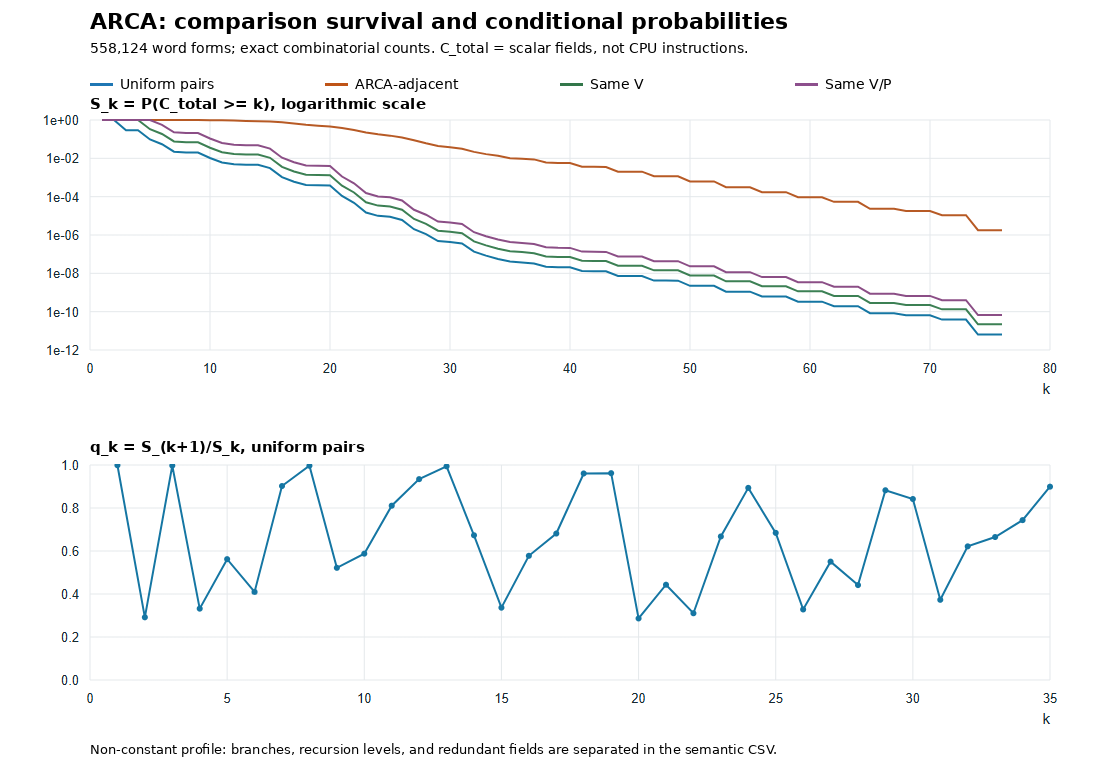
\includegraphics[width=0.96\textwidth]{q_profile_en.png}
\caption{Empirical survival profiles $S_k$ and conditional probabilities $q_k$ over the ARCA vocabulary. The ARCA-adjacent curve decays much more slowly than the uniform-pair curve, indicating significantly longer shared structural prefixes.}
\label{fig:profilo-q}
\end{figure}

\subsection{Semantically interpretable probabilities}

The positional profile $q_k$ can be complemented by conditional probabilities associated with the different structural stages. At the first recursive level, over the corpus under consideration, the values in Table~\ref{tab:q-semantiche} are observed.

\begin{table}[htbp]
\centering
\caption{First semantically interpretable conditional probabilities.}
\label{tab:q-semantiche}
\begin{tabular}{lrrr}
\toprule
Stage & Incoming pairs & Continuing pairs & $q$ \\
\midrule
Final vowel $V$ & 155590780366 & 45367372759 & 0.291581 \\
Pivot state $\tau$ & 45367372759 & 45239410378 & 0.997179 \\
Pivot vowel $P$ & 45239286624 & 15019564687 & 0.332003 \\
Gap $G$ & 15019564687 & 8441938139 & 0.562063 \\
First internal letter $I_1$ & 8441938139 & 3456604528 & 0.409456 \\
\bottomrule
\end{tabular}
\end{table}

For example, $q_V\simeq0.2916$ means that, among the pairs entering the first vocalic level, approximately $29.16\%$ share the final vowel; $q_P\simeq0.3320$ means that, after the preceding checks have been passed and when both pivots exist, about one third of the pairs also share the pivot vowel. These values must not be multiplied indiscriminately across stages belonging to different branches: the complete $q_k$ profile follows the actual field order, whereas the quantities in the table mainly serve an interpretive purpose.

At subsequent recursive levels, comparison of the current final vowel has conditional probability $1$, because it coincides with the pivot already found equal at the previous level. This example shows why a single constant $q$ does not adequately describe actual behavior: some discriminants contribute new information, while others are deterministic consequences of the recursion.

\subsection{Sorting a vocabulary}

Let $M$ be the number of words and
\[
  N=\sum_{j=1}^{M}|w_j|
\]
the total size of the vocabulary in characters. Precomputing all signatures costs $\Theta(N)$. A comparison-based sorting algorithm performs $O(M\log M)$ comparisons; in the worst case, if each comparison costs $O(L)$, the simple bound is
\[
  O(N+ML\log M).
\]

It is not correct, however, to automatically multiply $M\log M$ by the mean value of $C$ computed for uniform pairs: a sorting algorithm chooses pairs adaptively and the distribution of comparisons actually performed is different. In the benchmark, for example, the real sort trace with the flat signature has mean cost $C_{\mathrm{total}}\simeq10.52$, much greater than the value $2.83$ for uniform pairs. Any average-case complexity analysis of sorting therefore requires a model specific to the comparison stream of the algorithm used.

\subsection{Contiguity of structural prefixes}

Here the most important property for using the ordering as an index emerges.

\begin{proposition}[Contiguity of a prefix-defined class]
Let $\alpha$ be a prefix of the complete key $K$, and let
\[
  A_{\alpha}=\{w:K(w)\text{ begins with }\alpha\}.
\]
In any list ordered lexicographically according to $K$, the elements of $A_{\alpha}$ form a contiguous interval.
\end{proposition}

\begin{proof}
Let $u,v\in A_{\alpha}$ with $K(u)\lexord K(v)$, and let $z$ be a word such that
\[
  K(u)\lexord K(z)\lexord K(v).
\]
Suppose for contradiction that $K(z)$ does not begin with $\alpha$. Let $j$ be the first position, within the length of $\alpha$, at which $K(z)$ differs from $\alpha$. All preceding positions coincide. If the field of $K(z)$ at position $j$ were smaller than the corresponding field of $\alpha$, then $K(z)$ would precede every key beginning with $\alpha$, in particular $K(u)$; if it were greater, it would follow every such key, in particular $K(v)$. Both cases contradict the hypothesis. Therefore $K(z)$ must begin with $\alpha$ and belongs to $A_{\alpha}$.
\end{proof}

\begin{corollary}[Searching a structural interval]
In a vocabulary of $M$ words ordered according to $K$, the endpoints of a class defined by a structural prefix can be found with two binary searches. If the prefix length is $t$ and the class contains $k$ results, the cost is
\[
  O(t\log M+k),
\]
which becomes $O(\log M+k)$ when $t$ can be treated as a constant or prefix comparison is precomputed. In the general case in which one comparison may require $O(L)$, the corresponding bound is $O(L\log M+k)$.
\end{corollary}

In left-to-right alphabetical order, a property depending on the ending or on vocalic structure does not in general have this contiguity property. In the absence of an auxiliary index, there are therefore instances in which $\Theta(M)$ words must be inspected to enumerate all matches. Similarly, reverse ordering is particularly well suited to exact literal suffixes, which become prefixes of the reversed strings.

\subsection{Rhymes, assonances, structural form, and consonances}

To distinguish the behavior of different properties, the benchmark considered several experimental graphemic classes. They are not universal linguistic definitions of rhyme, assonance, or consonance; they serve to measure how closely a property is aligned with the primary ordering.

In particular:
\begin{itemize}
  \item an exact literal suffix is naturally aligned with reverse lexicographic order;
  \item the pair ``final vowel + pivot vowel'', requiring the presence of a pivot, is a prefix of the ARCA signature and provides a simple proxy for \emph{structural assonance};
  \item adding the gap yields a \emph{structural-form} class that is still prefix-defined;
  \item fixing the entire local record of the first wagon yields a more specific structural prefix;
  \item a consonantal proxy obtained by ignoring the endpoint vowels and retaining the internal consonants is not, in general, a prefix of the ARCA signature.
\end{itemize}

Table~\ref{tab:contiguita} reports the minimum, median, and maximum number of intervals required to represent each class over the complete vocabulary, not merely over a sample of queries.

\begin{table}[htbp]
\centering
\caption{Contiguity of experimental classes under the three orderings. Triples report minimum/median/maximum number of intervals per class.}
\label{tab:contiguita}
\resizebox{\textwidth}{!}{%
\begin{tabular}{lrrrrl}
\toprule
Family & Classes & Word forms & ARCA & Alphabetical & Reverse \\
\midrule
Final vowel + pivot & 25 & 556770 & 1 / 1 / 1 & 35 / 11478 / 69261 & 26 / 256 / 404 \\
Final vowel + pivot + gap & 118 & 556770 & 1 / 1 / 1 & 1 / 148 / 55210 & 1 / 36.5 / 229 \\
Complete first wagon & 4468 & 556770 & 1 / 1 / 1 & 1 / 3 / 32936 & 1 / 1 / 10 \\
Consonantal proxy & 417 & 556770 & 1 / 2 / 89 & 1 / 2 / 54940 & 1 / 2 / 161 \\
\bottomrule
\end{tabular}%
}
\end{table}

The first three families are prefixes of the signature and, consistently with the contiguity proposition, all their classes occupy a single ARCA interval. The empirical result therefore verifies, over the complete corpus, that the concrete implementation realizes the property predicted by the theory. The consonantal proxy, which is not a prefix of the signature, may instead require up to $89$ ARCA intervals; for this property no uniform superiority emerges, and an additional index may be appropriate.

These results clarify the role of the ordering. ARCA is not a universally better replacement for alphabetical or reverse order: alphabetical order remains natural for literal prefixes, and reverse order for exact suffixes. ARCA's specific advantage concerns properties that become prefixes of its structural representation, especially those based on the hierarchy final vowel--pivot--gap--wagon interior.

\subsection{Empirical interpretation of structural clustering}

The strong difference between uniform pairs and adjacent pairs provides a second verification, distinct from contiguity. Two words chosen uniformly from the vocabulary are separated on average after about $2.83$ fields; two words made adjacent by the ARCA ordering instead require about $19.14$ fields. This means that adjacent elements of the ordering share, on average, much longer prefixes of the signature.

This behavior provides internal empirical evidence that the ordering achieves the goal for which it was defined: placing near one another words that share a larger amount of ARCA structure. By itself, it does not prove that such words are necessarily more similar under every phonetic, perceptual, or poetic notion of similarity; it does show, however, that the mathematical notion of proximity induced by the signature is effectively reflected in the resulting ordering.

\section{Graphemic nature and limitations}

The basic construction operates on spellings, not directly on phonemes. It must therefore not be interpreted as a universal linguistic definition of rhyme, assonance, or consonance. In Italian, the relationship between spelling and pronunciation is often informative but not perfect; homographs, unwritten stress, loanwords, and other irregularities may produce divergences.

The method should therefore be understood as a graphemic structural representation oriented toward sound-based literary exploration, potentially extensible in the future with phonetic or prosodic information.

\section{Conclusions}

The ARCA method associates a word with a recursive structure determined by its vowels and by the distances between them. At each level, the notion of pivot identifies the first vowel that is non-adjacent to the current final vowel; the segment delimited by the pivot and the final vowel forms a wagon; the pivot then becomes the final vowel of the next level. The procedure always terminates and produces a finite structural signature.

From this signature, completed by class indicators and deterministic tie-breakers, one obtains a strict total order on words. The construction differs from a simple reverse dictionary because the priority order depends on the vocalic structure of the word rather than only on the geometric distance of characters from the end.

From a computational standpoint, the signature can be built in linear time; comparison between precomputed signatures is constant in the best case and linear in the worst case. Average behavior can be described without imposing a single continuation constant, using the survival function $S_k$ and the conditional probabilities $q_k$. The geometric bound with a constant $q<1$ remains an abstract corollary, but the census of the vocabulary shows that the different stages have different behaviors and that some recursive comparisons are deterministically redundant.

The most relevant result for search is the contiguity of classes defined by prefixes of the structural key. In the current ARCA vocabulary, all observed classes defined by final vowel and pivot, by final vowel--pivot--gap, and by the complete first wagon form a single interval in the ordering. Moreover, ARCA-adjacent pairs require on average about $19.14$ fields to be distinguished, compared with about $2.83$ for uniform pairs: this provides empirical evidence that the ordering effectively clusters word forms sharing a greater amount of the structure for which it was designed. This result concerns the mathematical proximity induced by the signature and must not be confused with a universal definition of phonetic or poetic similarity.

\section*{Authorship, license, and citation note}

The idea of the ordering, the terminology of \emph{pivot} and \emph{wagon}, and the project direction of the ARCA method are by Luca Montanelli. The formalization and technical writing were developed with the assistance of OpenAI artificial-intelligence tools, used to support discussion, verification, and drafting, not as authors of the work.

The text and formalization expressed in this document are intended to be released under the \textbf{Creative Commons Attribution 4.0 International (CC BY 4.0)} license. This license concerns the expressive content of the document and does not purport to create an exclusive right over the abstract mathematical idea itself.

For academic uses, derivative software, or works that explicitly employ the ARCA method, citation of this document is requested. A definitive bibliographic citation and DOI may be added when the stable version is published.

\section*{Acknowledgments}

The author thanks Carlo Barabucci for the program \emph{Anagrammi e non solo}, which provided an important technical basis for the subsequent evolution of the ARCA project.

\begin{thebibliography}{9}

\bibitem{crifo2011}
F. Crifò,
\emph{Rimari e dizionari inversi},
Enciclopedia dell'Italiano, Treccani, 2011.
\url{https://www.treccani.it/enciclopedia/rimari-e-dizionari-inversi_%28Enciclopedia-dell%27Italiano%29/}

\bibitem{byrdchodorow1985}
R. J. Byrd and M. S. Chodorow,
\emph{Using an On-Line Dictionary to Find Rhyming Words and Pronunciations for Unknown Words},
Proceedings of the 23rd Annual Meeting of the Association for Computational Linguistics, pp. 277--283, 1985.
DOI: \href{https://doi.org/10.3115/981210.981244}{10.3115/981210.981244}.

\bibitem{boudelaa2004}
S. Boudelaa and W. D. Marslen-Wilson,
\emph{Abstract morphemes and lexical representation: the CV-Skeleton in Arabic},
Cognition, 92(3), pp. 271--303, 2004.
DOI: \href{https://doi.org/10.1016/j.cognition.2003.08.003}{10.1016/j.cognition.2003.08.003}.

\bibitem{masterwriter2005}
B. Devorzon, M. Towers and S. Vanderbilt,
\emph{An information management system plus},
European patent application EP1581892A1, publication 2005.

\end{thebibliography}

\end{document}
